
  For the studies of the Higgs boson in which we wish to claim that precisely measured deviations from the SM can give a discovery of new physics, we must be certain that systematic errors are both small and well-constrained.  In this section, we will discuss 
the sources of systematic error that we consider in our Higgs coupling analysis.

A general statement is that it is important to measure effects correlated to systematic uncertainties.  For this, it is crucial to always have one more degree of freedom that (statistically) absolutely required.  In the ILC program, electron and positron polarisation
provide tools to validate estimates of systematic errors, and to reduce these 
sources of uncertainty.  In Sec.~\ref{subsec:beampol}, when we reviewed in general terms the importance of the
 use of beam polarisation to meet the physics goals of the ILC, we did not emphasize this 
aspect of the physics implication of polarisation.  But it is clear that, for each measurement that can be done at an unpolarized collider, a collider with control of the polarization for each beam can provide four independent data sets.  We will explain in this section how this tool 
can be used not only to estimate but also to reduce systematic errors.



\subsubsection{Systematic uncertainties considered in the Higgs coupling fit}
\label{subsubsec:sysuncert}
The evaluation of systematic uncertainties for experiments which have not yet been built is a difficult task and will to some extent always remain guess-work until real data have been taken. To some extent, we can rely on the experience from previous $e^+e^-$ experiments, especially at LEP, where many uncertainties could be controlled to a typical level of 1\%.
The ILC detector designs, which aim for higher precision, make use of this experience,
as explained in Sec.~\ref{sec:detectors}.  Assuming this basic level of performance, detailed studies of systematic uncertainties at the ILC have concentrated on cases where the statistical uncertainties are expected to be significantly below 1\%, and on searches in channels with large irreducible backgrounds. An example for the first case is a global analysis of total rates and differential distributions of various 2-fermion and 4-fermion SM processes, extracting simultaneously the total unpolarised cross sections, the relevant left-right asymmetries, the beam polariations and the charged triple gauge couplings, see Sec.~\ref{subsec:ew_WWana} and Ref.~\cite{bib:PhDRobert}. An illustrative example for the second category, though not directly connected to Higgs physics, is the WIMP search in the mono-photon channel, see Sec.~\ref{sec:searches} and Ref.~\cite{Habermehl:417605}. 

Studies of this type lead us to the following estimates of the dominant systematic uncertainties (previewed already at the end of Sec.~\ref{subsec:higgs_ana}:
\begin{itemize}
\item The luminosity at the ILC will be measured from low-angle Bhabha scattering with the help of a dedicated forward calorimeters, the LumiCals (see Sec.~\ref{subsub:det:forward} and Ref.~\cite{Abramowicz:2010bg}). This measurement is extremely sensitive to the exact alignment of the LumiCals on the two sides of the detector, as well as to beam backgrounds and has been studied in detailed simulations both for the ILC and for CLIC~\cite{Bozovic-Jelisavcic:2014aza, Lukic:2013fw}. Based on these studies, the resulting systematic uncertainty on all Higgs cross section and cross-section-times-braching-ratio measurements is assumed to be 0.1\%
\item Another 0.1\% is assumed for the net systematic effect of the finite knowledge of luminosity-weighted long-term average values of the beam polarisations at the $e^+e^-$ interaction point. While the Compton polarimeters in the Beam Delivery System resolve time-dependencies at the level of 0.25\%~\cite{Vormwald:2015hla, List:2015lsa}, also the effects of spin transport, misalignment of beam line magnets as well as depolarisation during the beam-beam interaction have been studied~\cite{Beckmann:2014mka}. The absolute scale of the luminosity-weighted average polarisation at the IP is finally calibrated from collision data, \eg, from a global fit SM processes with a strong polarisation dependence~\cite{bib:PhDRobert}. 
\item Theoretical uncertainties are also assumed to have reched at the level of 0.1\% by the time of ILC operation.   This requires the computation of all relevant processes to 2 loops in the electroweak interactions, a task feasible within the current state of the art~\cite{Blondel:2019qlh}.  Another question is the availability of high-precision values for the most important input parameters---$m_b$, $m_c$, $\alpha_s$, and $m_h$.  We expect to obtain the first threee  of these to sufficient accuracy from lattice QCD~\cite{Lepage:2014fla}.
For $m_h$, the  ILC recoil measurement described in Sec.~\ref{sec:higgs:sigmazh} will provide 
the high precision needed.
\item For flavor tagging, systematic errors of 1\% have already been reached at LEP.. With the advances in detector technology and the larger integrated luminosity, we assume that for each data set at the ILC this can be reduced  and also improved as  a function of integrated luminosity by probe-and-tag measurements.   We expect an uncertainty of 
$0.3\% \sqrt{0.250/L}$, where $L$ is the integrated luminosity in iab.  This is an error of 0.1\% for the ILC250.
% , improving  These 0.3\% are considered as net effect of all experimental uncertainties in the absence of beam polarisation.

% In the presence of both beam polarisations, the net effect of systematic uncertainties has been shown to be smaller by factors between 2 and 10 due to the correlations between data sets with different beam polarisations as discussed in Sec.~\ref{subsubsec:pol:systematics}. Since the Higgs coupling fit does not yet comprise such a detailed treatment of systematic uncertainties and their correlations as the above mentioned global fit to 2-fermion and 4-fermion processes, we assume that, in presence of polarised beams, the net effect of the experimental uncertainties reduces to 0.1\%.

The same uncertainties have been considered in projections of triple gauge coupling precisions in full simulation of the ILD detector, c.f.\ section~\ref{subsec:ew_WWana}.

\end{itemize}



\subsubsection{Control of systematic uncertainties using beam polarisation} 
\label{subsubsec:pol:systematics}

In the remainder of this section we will highlight the impact of the beam polarisation on the control of systematic uncertainties using these two studies as examples.   We have already pointed out that beam polarisation provides subsets of the data that can be used as cross-checks of systematic errors on 
efficiencies for signal identification and background suppression.  However, the studies
in Refs.~\cite{bib:PhDRobert} and \cite{Habermehl:417605} go beyond this to illustrate the use of beam polarisation to actually reduce systematic errors beyond what is possible at 
an unpolarised collider.   Both of these studies were carried out for measurements at the 
500~GeV ILC, but the same principles apply to the 250~GeV data.

Several principles combine to produce this  result.   The first is that different polarization
settings produce event samples with different mixtures of signal and background 
processes.   The differences in these  mixtures arise from order-1 polarization asymmetries that vary from 
process to process, to first approximation, in the manner predicted by the SM.   In the SM, for example, lepton pair production has a small polarization asymmetry while the   polarization asymmetry for $b\bar b $ production is large and that for $W$ pair production is almost maximal.   For certain modes, for example, lepton pair production and di-jet production, the detection  efficiency is naturally very high and therefore has a small uncertainty, while, for other processes, for example, $b\bar b$ production, this efficiency is smaller and also more complicated to estimate.  If we introduce nuisance factors for the more uncertain efficiencies
and determine these from data, the correlation of the relative compositions with polarization
allows us to determine these parameters in terms of the efficiencies that are better known. 

The second principle is that systematic uncertainties that are correlated with polarization can be cancelled locally in the data set using fast reversal of the beam helicities.  This principle 
was essential to the excellent measurement of $\sin^2\theta_w$ by the SLD experiment 
from a very small data sets; almost all systematic errors were cancelled by flipping the $e^-$ beam  polarization in a pseudo-random fashion~\cite{Abe:1996nj}.   The principle of rapid helicity reversal is built into the ILC design, which give the capability to flip the sign of 
polarisation for each of the two beams independently on a train-by-train basis (see Sec.~\ref{par:beampol}.  This helicity reversal is fast compared to typical time-scales of changes in the configuration, calibration, and alignment of the detector and the accelerator.
It implies that data sets with the same beam energy but different beam helicities can be considered as being collected  essentially concurrently.  

%%%%%%%%%%%%%%%%%%%%%%%%%%%%%%%%%%%%
\begin{figure}
\centering
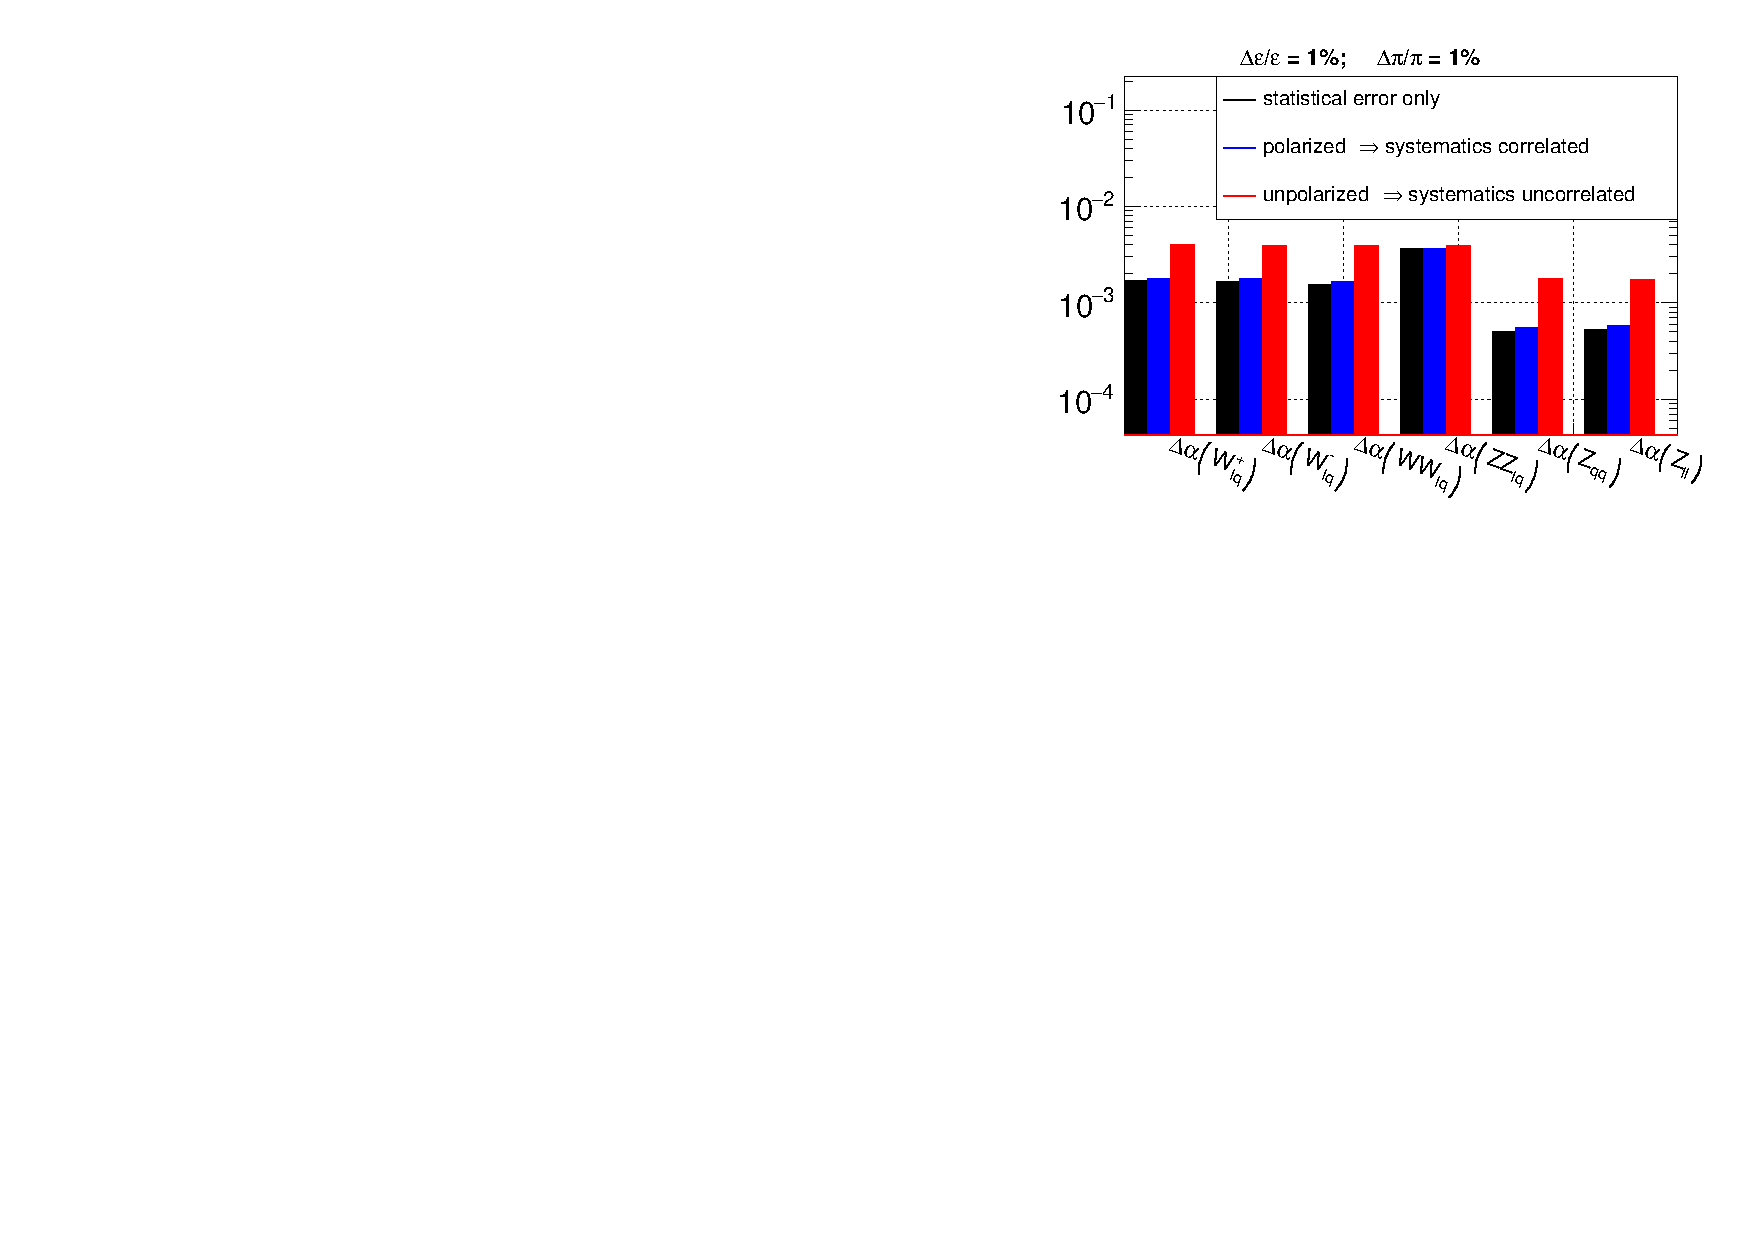
\includegraphics[width=0.95\linewidth]{./chapters/figures/ElectroWeakSysDependency_alpha_short.pdf}
		
\caption{Uncertainties on the unpolarised cross sections of various 2-fermion and 4-fermion processes as obtained from the global fit introduced in the text~\cite{bib:PhDRobert}, assuming a systematic uncertainty of 1\% on the selection efficiencies and purities, each. In the case of polarised beams, it is assumed that only 10\% of the uncertainty is uncorrelated between data sets - in this case the impact of the systematic uncertainties is minimal. Without the redundancies provided by data sets with correlated systematic uncertainties, the total uncertainties increase by a factor 2 for $WW$ and single-$W$ processes and a factor of 5 for 2-fermion processes.}
\label{fig:alpha_error_corr_uncorr}
\end{figure}
%%%%%%%%%%%%%%%%%%%%%%%%%%%%%%%%%%%%%%


The improvement in the measurement of the absolute normalization of cross sections can be very significant.  The study of Ref.~\cite{bib:PhDRobert} considered the full set of 2-fermion production processes and 4-fermion production processes (including $\ee\to WW / ZZ \to 4$~fermions and well as single-$W$ production) at 250~GeV.   Each channel was assigned a 1\% systematic uncertainty in its selection efficiency and signal purity. Based on the correlations of experimental effects between ``quasi-concurrently'' taken data sets, discussed in section~\ref{subsubsec:pol:systematics}, it was assumed that only 10\% of this uncertainty is uncorrelated between data sets with different the beam polarisation configurations. Thus, a global fit using all four
polarization settings allows one to determine the relative efficiencies and remove most of the systematic uncertainty.  The result for the final normalization uncertainties are shown in 
Fig.~\ref{fig:alpha_error_corr_uncorr}.  For each of several 2- and 4-fermion channels, the black bars should the statistical uncertainties, the red bars show the full uncertainties for unpolarised data, and the blue bars show the uncertainties for polarised data samples.   The final uncertainties are larger in unpolarized case by a factor of 2 for $WW$ and single-$W$ processes and by a factor of 5 for lepton pair production.

%%%%%%%%%%%%%%%%%%%%%%%%%%%%%%%%%%%%%%%%%%%%%%
\begin{figure}
\centering
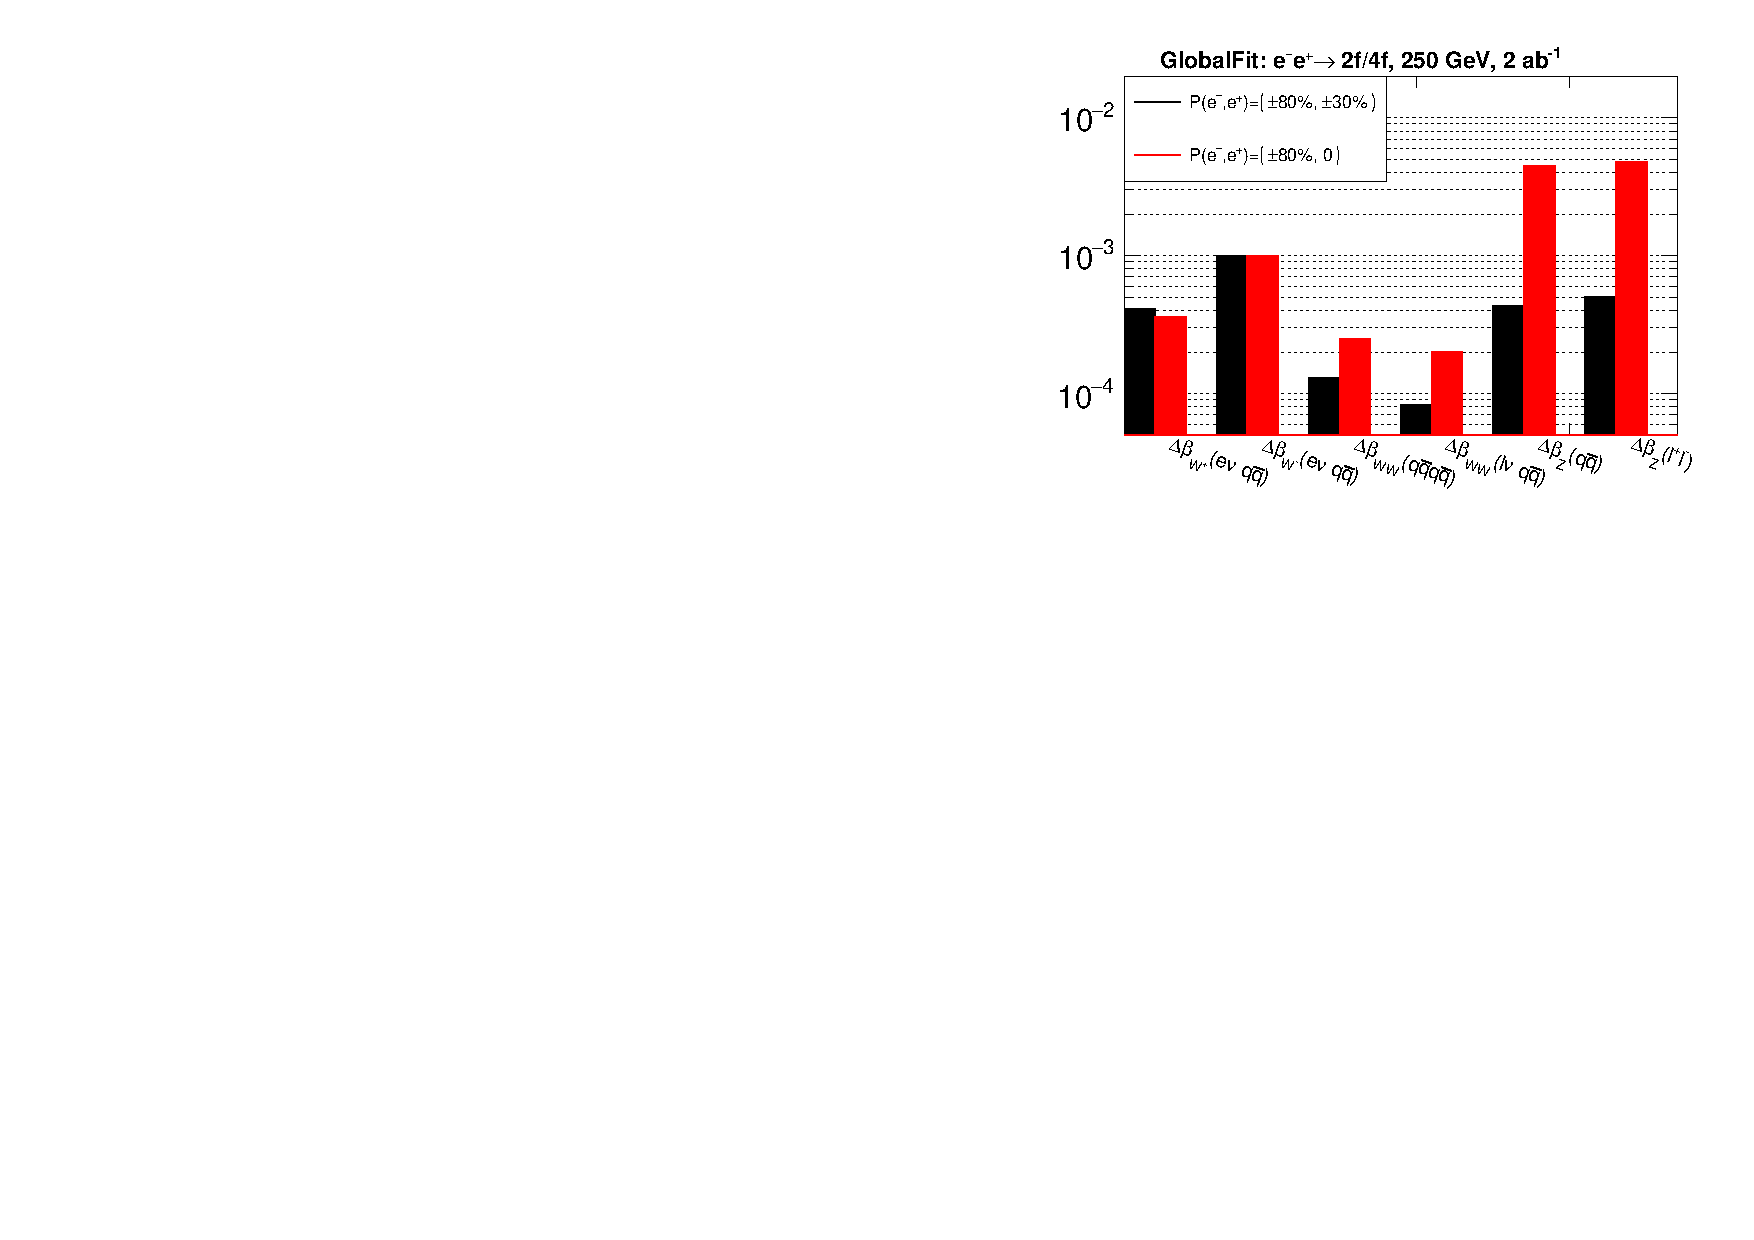
\includegraphics[width=0.95\linewidth]{./chapters/figures/beta_precision_upolarized.pdf}
		
\caption{Uncertainties $\Delta \beta$ on \ALR\ of various 2-fermion and 4-fermion processes as obtained from the global fit introduced in the text~\cite{bib:PhDRobert} with both beams polarised (with the standard 45\%/45\%/5\%/5\% sharing between the four helicity configurations) and in the absence of positron polarisation (with a 50\%/50\% sharing between the two remaining helicity configurations). In the absence of positron polarisation, the  uncertainties on \ALR\ increase by a factor 2 for $WW$ and by about a factor of 10 for 2-fermion processes. Alone the single-$W$ processes remain unaffected.}
\label{fig:beta_error_noposipol}
\end{figure}
%%%%%%%%%%%%%%%%%%%%%%%%%%%%%%%%%%%%%%%%%%%%%%


The same principles can be applied to the measurement of polarisation asymmetries $A_{LR}$, which, as we have seen, play a large role in the ILC program.   Though many systematic 
errors automatically cancel in $A_{LR}$, there are new sources of systematic uncertainty, for example, the possibility of a correlation between the helicity orientation and the luminosity delivered per bunch train.   This is effectively controlled if both the electron and positron 
bunches can be polarised.  Roughly, the polarization asymmetry in $W$ pair production is almost maximal, and the small uncertainty in this quantity can be transferred to the value of $A{LR}$ for other processes. The point is illustrated in Fig.~\ref{fig:beta_error_noposipol}, again from Ref.~\cite{bib:PhDRobert}, which shows a comparison of the final uncertainty on 
$A_{LR}$ in a global fit between a collider with $e^-$ and $e^+$ polarization (black bars) and a collider with only $e^-$ polarization (red bars). The improvement is a factor of 10 for 
fermion pair production.  (In this illustrative study, the systematic errors from detector efficiency and theory are set equal to zero.) 

%%%%%%%%%%%%%%%%%%%%%%%%%%%%%%
\begin{figure}
\centering
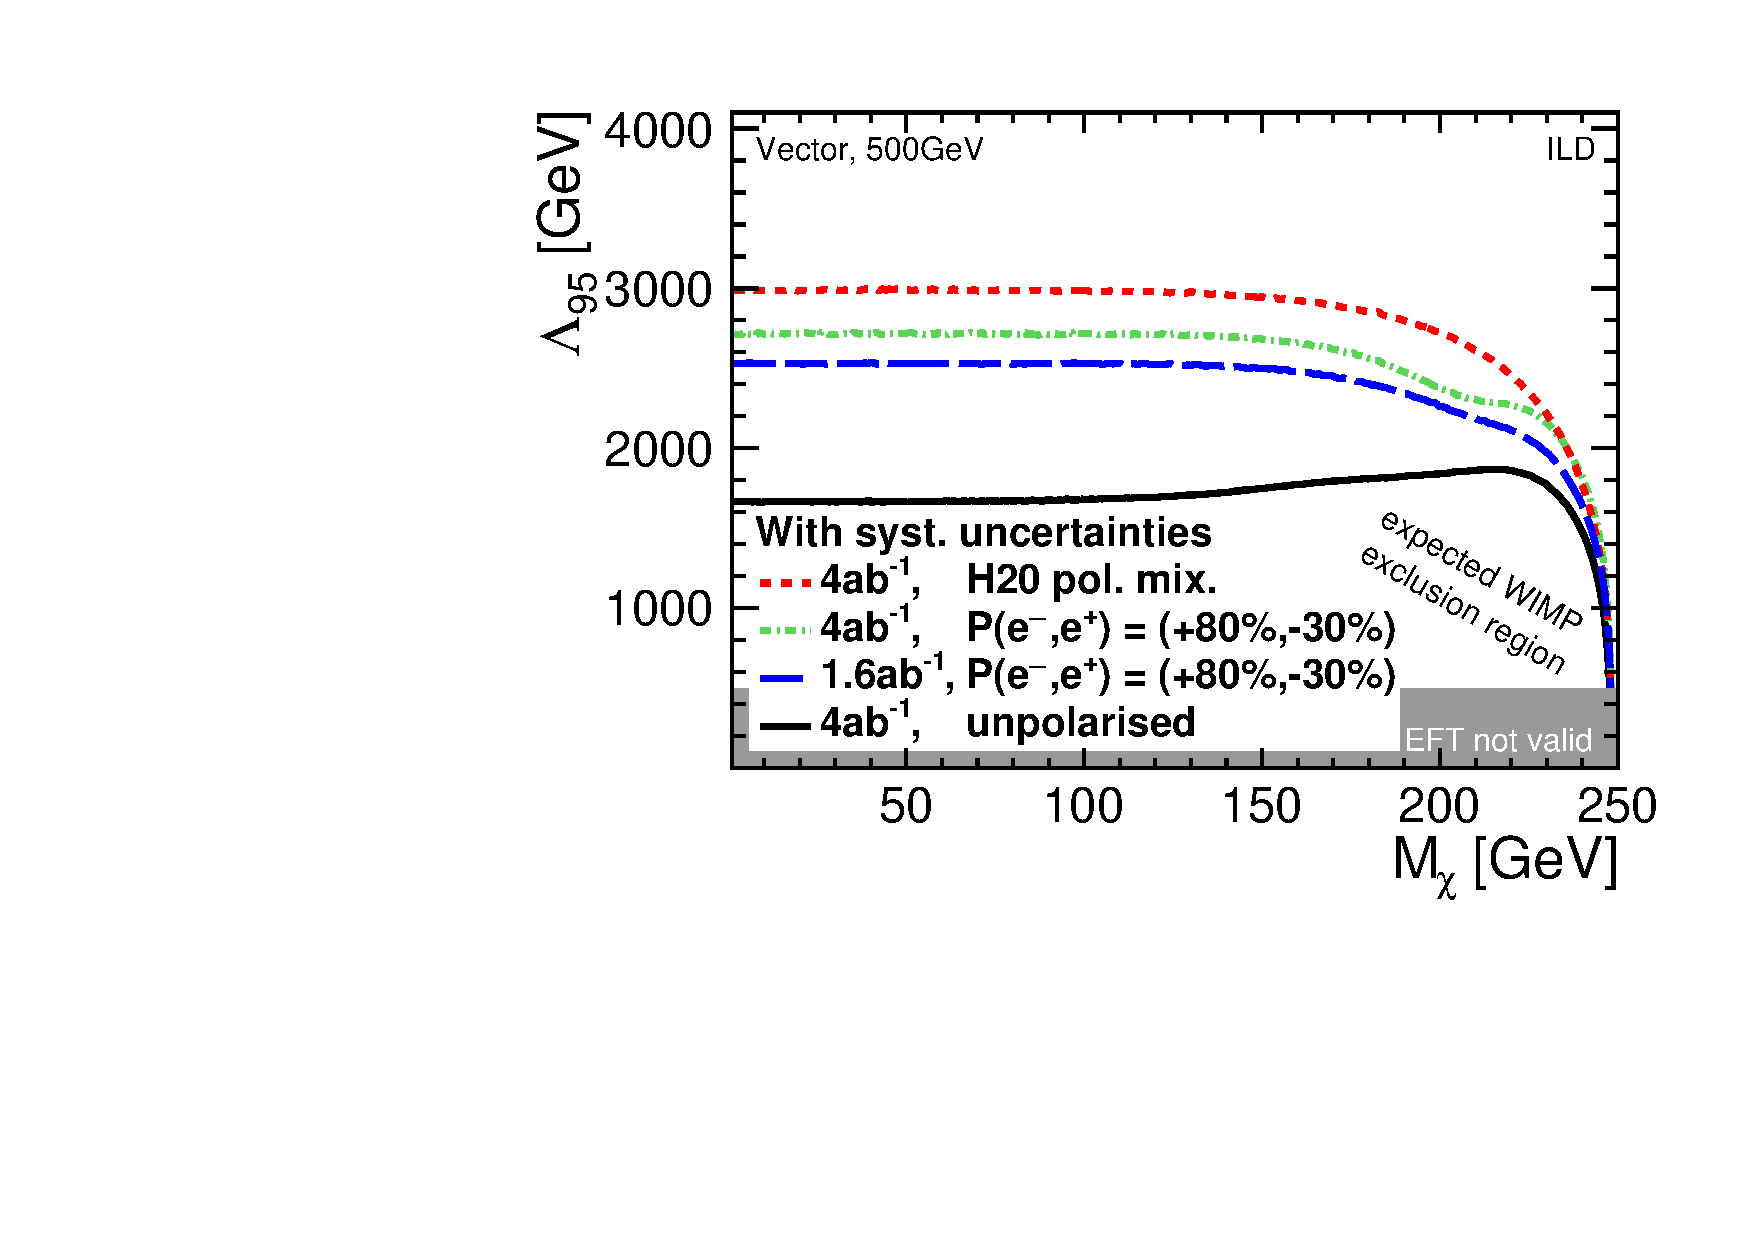
\includegraphics[width=0.95\linewidth]{./chapters/figures/vector_withSystematics.pdf}
		
\caption{Comparison of the reach of the search for WIMP production in the mono-photon channel for different assumptions on luminosity and polarization, {\em including} systematic uncertainties (see Sec.~\ref{sec:searches} for a description of the analysis)~\cite{Habermehl:417605}. }
\label{fig:polWIMPsys}
\end{figure}
%%%%%%%%%%%%%%%%%%%%%%%%%%%%%%%%%%%


Similar large effects from polarisation are seen in cases in which the signal is detected in 
the shape of  a  distribution.    An illustration here is given by a study of the search for 
dark matter particles $\chi$ using the mono-photon signature~\cite{Habermehl:417605}, already discussed in Sec.~\ref{subsec:beampol}.   In our earlier discussion, we pointed out that the signal from 
$\ee\to \gamma \chi\chi$ sits on top of a large irreducible background from 
$\ee\to \gamma \nu\bar \nu $.   the same study cases as Fig.~\ref{fig:polWIMPstat}. The study includes a careful evaluation of the systematic uncertainties, comprising those on selection efficiencies, luminosity, beam energy (spectrum) and polarization as well as on the theoretical modelling of the background. 
The limit calculation uses fractional event counting based on the observed energy spectrum of the selected photon candidates and considers normalisation and shape-dependent uncertainties as well as the correlations between these. If the mass of the $\chi$ is relatively high, only low-energy photons can appear in the signal process.  Then the high-energy part of the photon spectrum can be used to determine nuisance parameters assigned to the 
polarization and efficiencies.  The results for the lower limit on the mediator scale, including 
systematic errors, are shown in Fig.~\ref{fig:polWIMPsys}. This figure should be compared to 
Fig.~\ref{fig:polWIMPstat}, in which systematic errors are set to zero.   Note that, in this case, the strongest limits are set using a mixture of beam polarizations (the dashed red curve in both cases) since this allows the systematic errors from beam polarisation to be better 
controlled.



[ A paragraph is needed explaining our treatment of unpolarized colliders in Sec. XI C.]








